\documentclass{article}[11pt]
\usepackage{amsmath,amssymb,amsthm}
\usepackage{graphicx}
\graphicspath{{../figures/}}
\begin{document}
\title{Interventions and Analysis}
\author{Ryo Kimura}
\date{}
\maketitle

\section{Interventions}
\subsection{Context}
%In our model, we considered the following interventions
%\begin{enumerate}
    %\item reduce entering LTBI by 100/75/50\%
    %\item reduce transmission by 100\%
    %\item reduce immigration by 75/50\%
    %\item increase (overall) LTBI treatment by 100/300\%
    %\item combinations of 3 and 4
    %\item combinations of 1 and 4
%\end{enumerate}
According to the article by Hill, Becerra, and Castro, foreign-born LTBI (latent tuberculosis infection) contributes significantly to TB (tuberculosis) incidence rates in the United States. Thus, we focus our attention on the cost effectiveness of reducing the number of foreign-born incoming LTBI cases.

The United States already screens for LTBI for immigrants, but does not require treatment. Thus, one way to reduce incoming LTBI cases is to offer treatment to such immigrants. However, this misses illegal immigrants, who may not enter the U.S. through traditional channels.

An alternative method is to invest in LTBI treatment programs abroad. This reduces the number of LTBI cases at the source, and (in theory) would also catch illegal immigrants.

\subsection{Methods}
In our model, we create separate compartments for foreign-borns and set different (but similar) transition rates between those compartments. An intervention is then represented by changing the parameters of the model. For example, the intervention in which we reduce the number of incoming LTBI cases can be modeled by reducing the rate at which FB LTBI cases enter the respective compartments..

\subsection{Results}
The results of this intervention are shown in figure \ref{fig:redEnLTBIIncGrouped}. There are several things to notice in these graphs. First, at high (but unrealistic) levels of intervention, the incidence rates drop dramatically, with 100\% reduction resulting in TB elimination from the foreign-born population. %Furthermore, even at low levels of interventions the reduction in cases is quite signifcant.

\begin{figure}
    \centering
    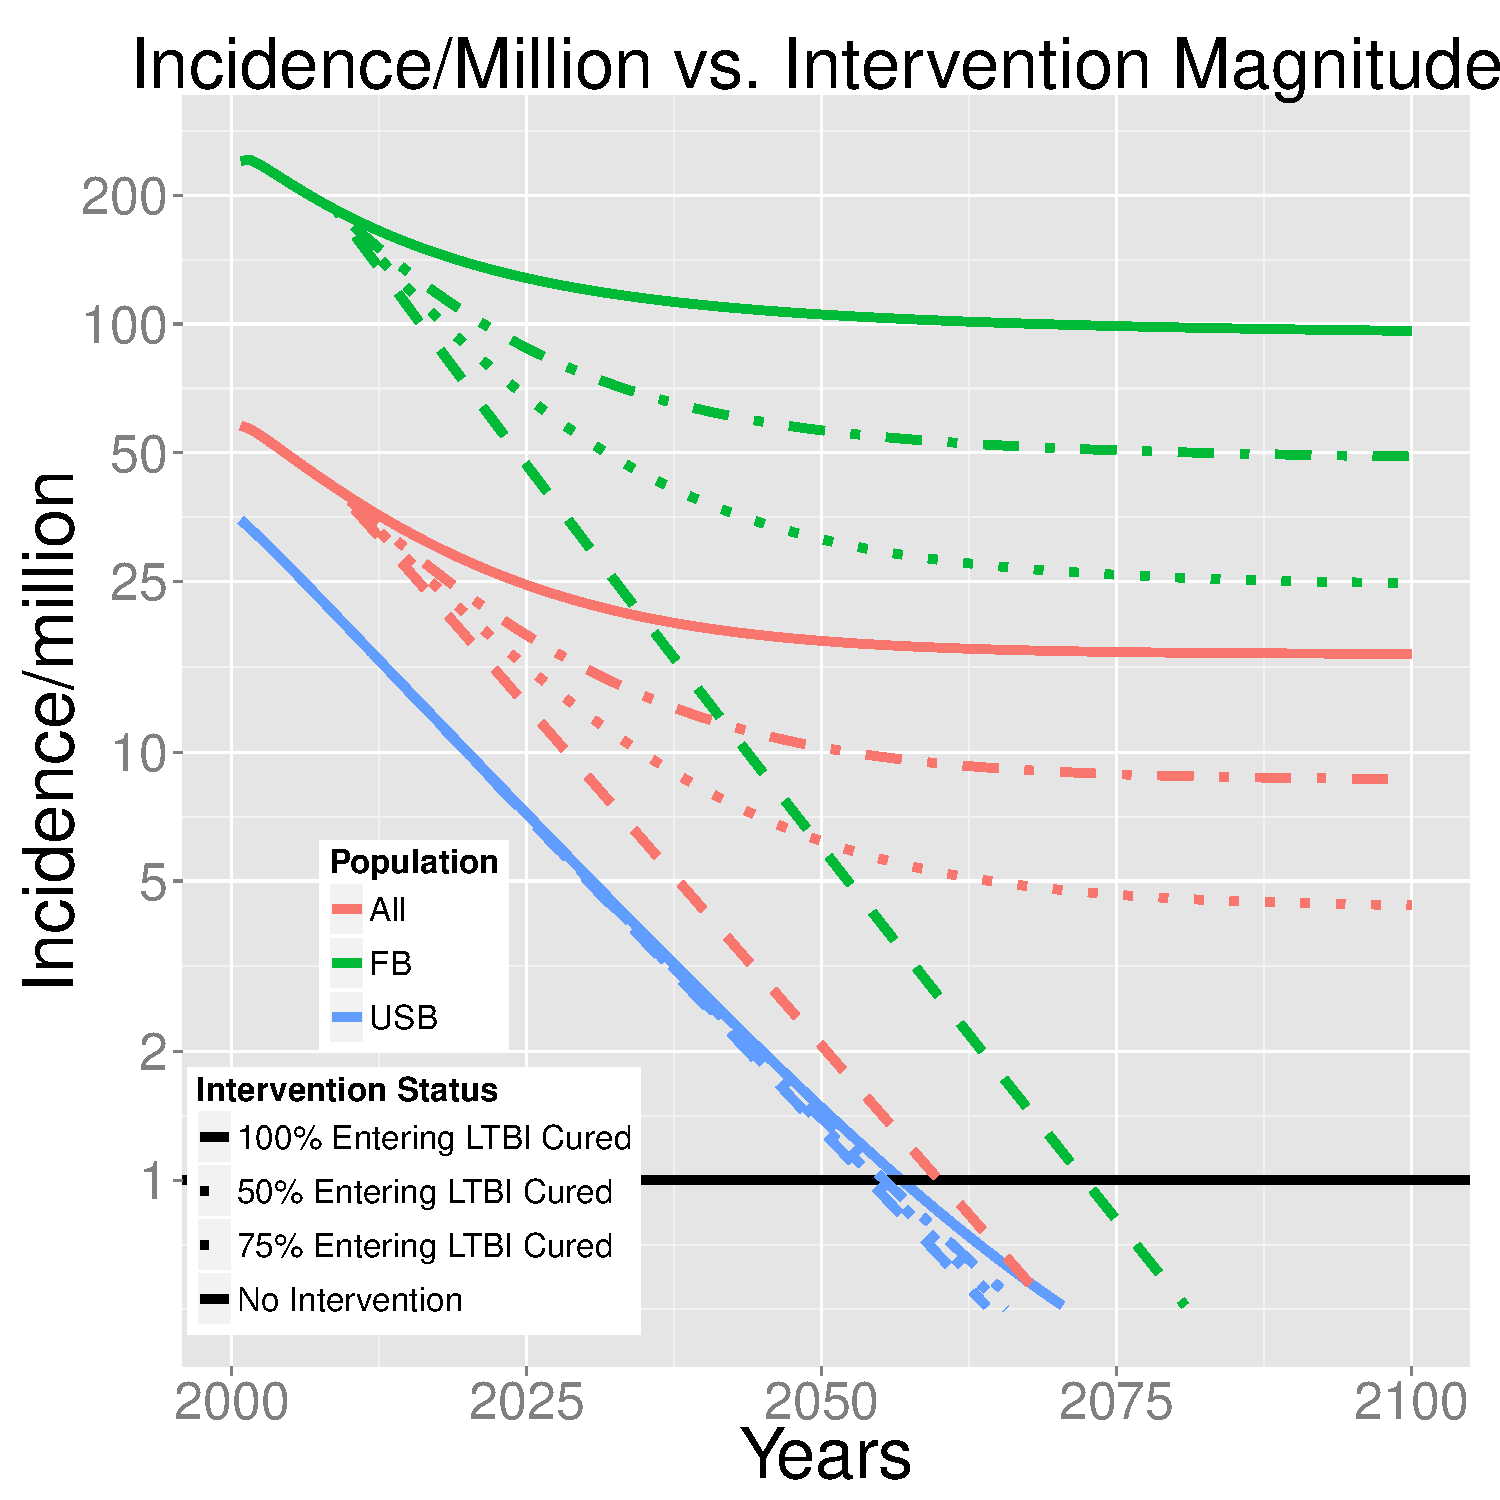
\includegraphics[width=3in]{redEnLTBIIncGrouped}
    \caption{Incidence/million With Reduced Incoming LTBI}
    \label{fig:redEnLTBIIncGrouped}
\end{figure}

The cost of these interventions is shown in figure \ref{fig:redEnLTBICostGrouped}. Here, the savings incurred from reducing incoming LTBI appears to grow linearly with respect to the size of the intervention. That is, if we cut the rate in half, then our cost (relative to the case in which we reduce the rate to zero) is also cut in half.

\begin{figure}
    \centering
    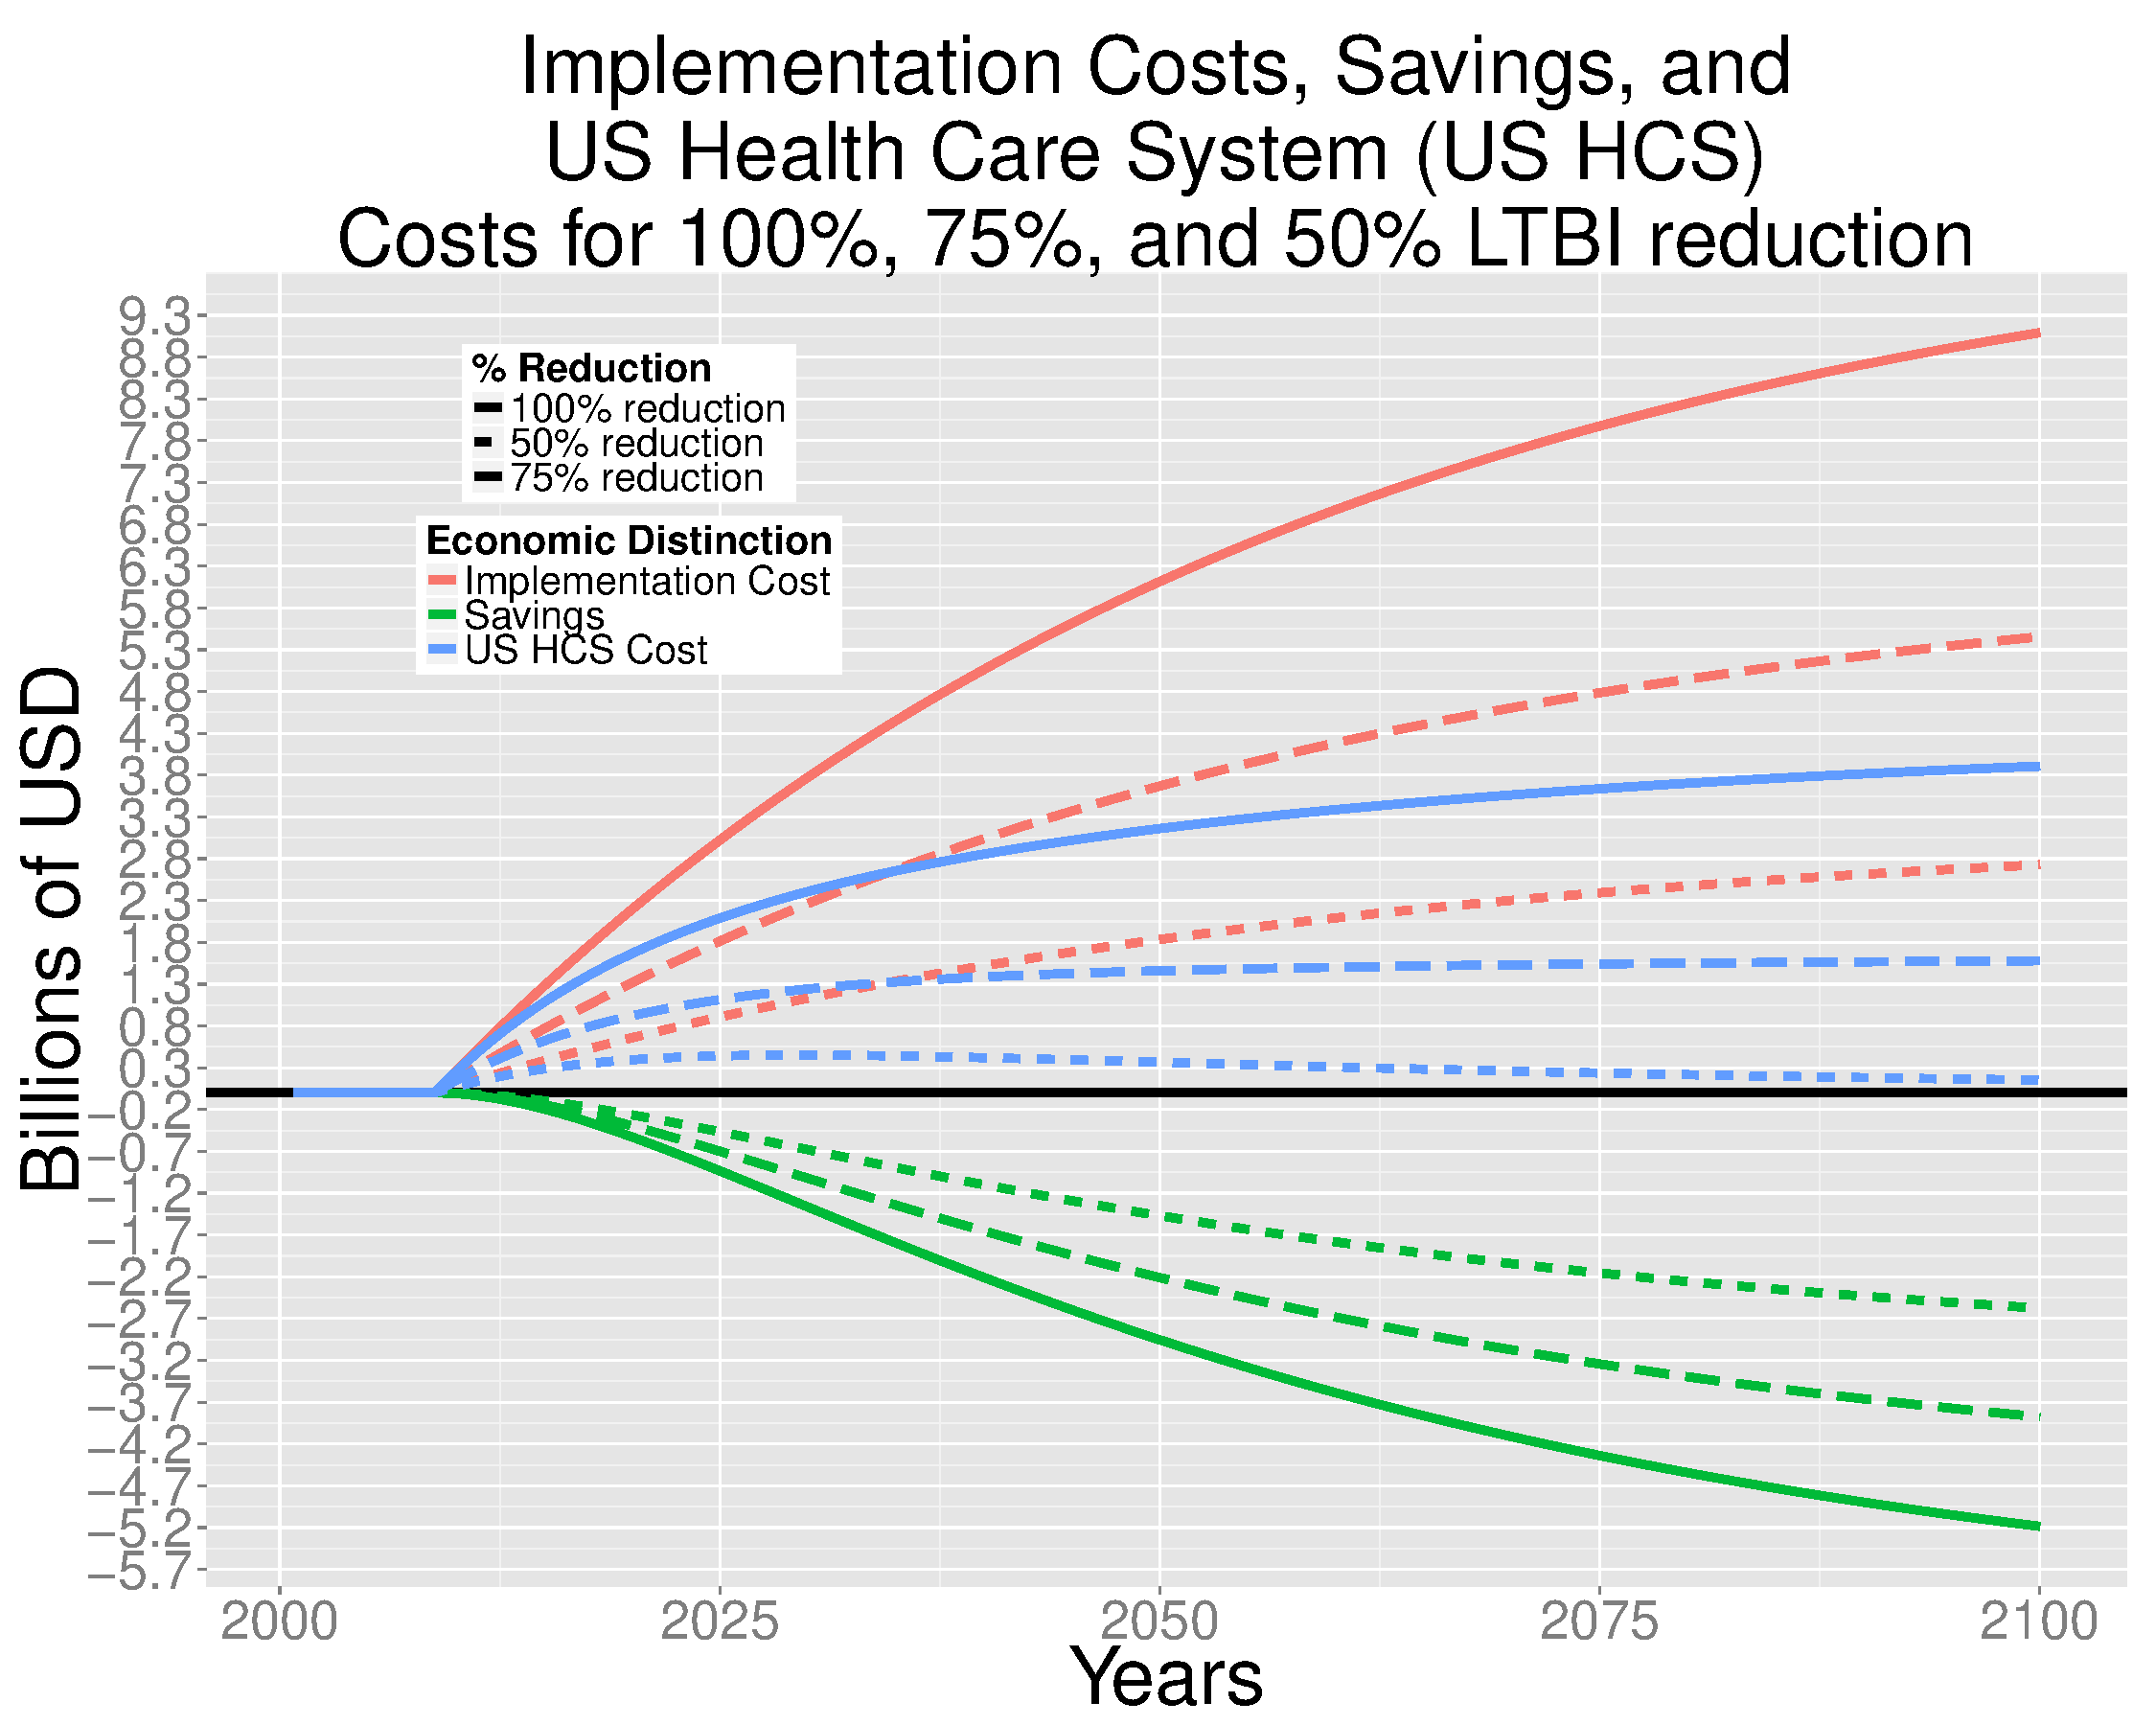
\includegraphics[width=3in]{redEnLTBICostGrouped}
    \caption{Total Cost of Reducing Incoming LTBI (over time)}
    \label{fig:redEnLTBICostGrouped}
\end{figure}

Table ?? summarizes the relative benefit of the cost when we reduce the number of incoming LTBI cases by 10\% (values for other interventions are listed in the supplement).

\subsection{Discussion}
As expected from the results of Hill et.al, reducing incoming LTBI has a significant impact on the TB incidence rate in the United States.
\end{document}
